\chapter{Дворовые компании\protect\footnote{Многие данные и фотографии предоставлены мне Т. В. Меньшиковой. Ей же благодарен за добрые советы.}}

Мне поручили написать о дворовых компанях, что я и постараюсь сделать с учетом <<собирательных>> свойств нашего Дома за период с тридцатых до шестидесятых годов. Аналог этого книжного варианта, естественно, будет в Альбоме.

Нельзя не сказать, что среди первопоселенцев нашего дома было очень много замечательных людей, начиная с Народного Комиссара иностранных дел М. М. Литвинова, его заместителей, руководителей подразделений, Чрезвычайных и полномочных посло того времени.

Сейчас, через 80 с лишним лет после заселения нашего дома, трудно сказать насколько были дружны между собой первопоселенцы, были ли дворовые компании у их старших детей (до 1920 года рождения)\footnote{Среди них, например: Клейн Н., Кунин В., Моргунова Т., рабинович Э., Рубинин П.}, привлекались ли в эти компании ребята из других домов, что было характерно для последующих поколений, когда компании формировались из ребят окрестных дворов, как правило, в возрастном диапазоне 2-3 года с вкраплениями до 5 лет.

Собирательная особенность нашего двора наметилась еще до Войны, у ребят около 1924 года рождения, в основном выпускников школ 1941 года. К ним относятся: Бабенко И. Я., Багун Ю. (воевал), Варзар Сева (прошел всю войну), Дивильковский Юра (погиб), Клейн Наташа (воевала), Короткин Жора (погиб), Кунина Ляля (воевала), миникс Аба (погиб).

\newpage % ??
\newgeometry{left=10mm, right=10mm, top=5mm, bottom=0mm}

\begin{center}
    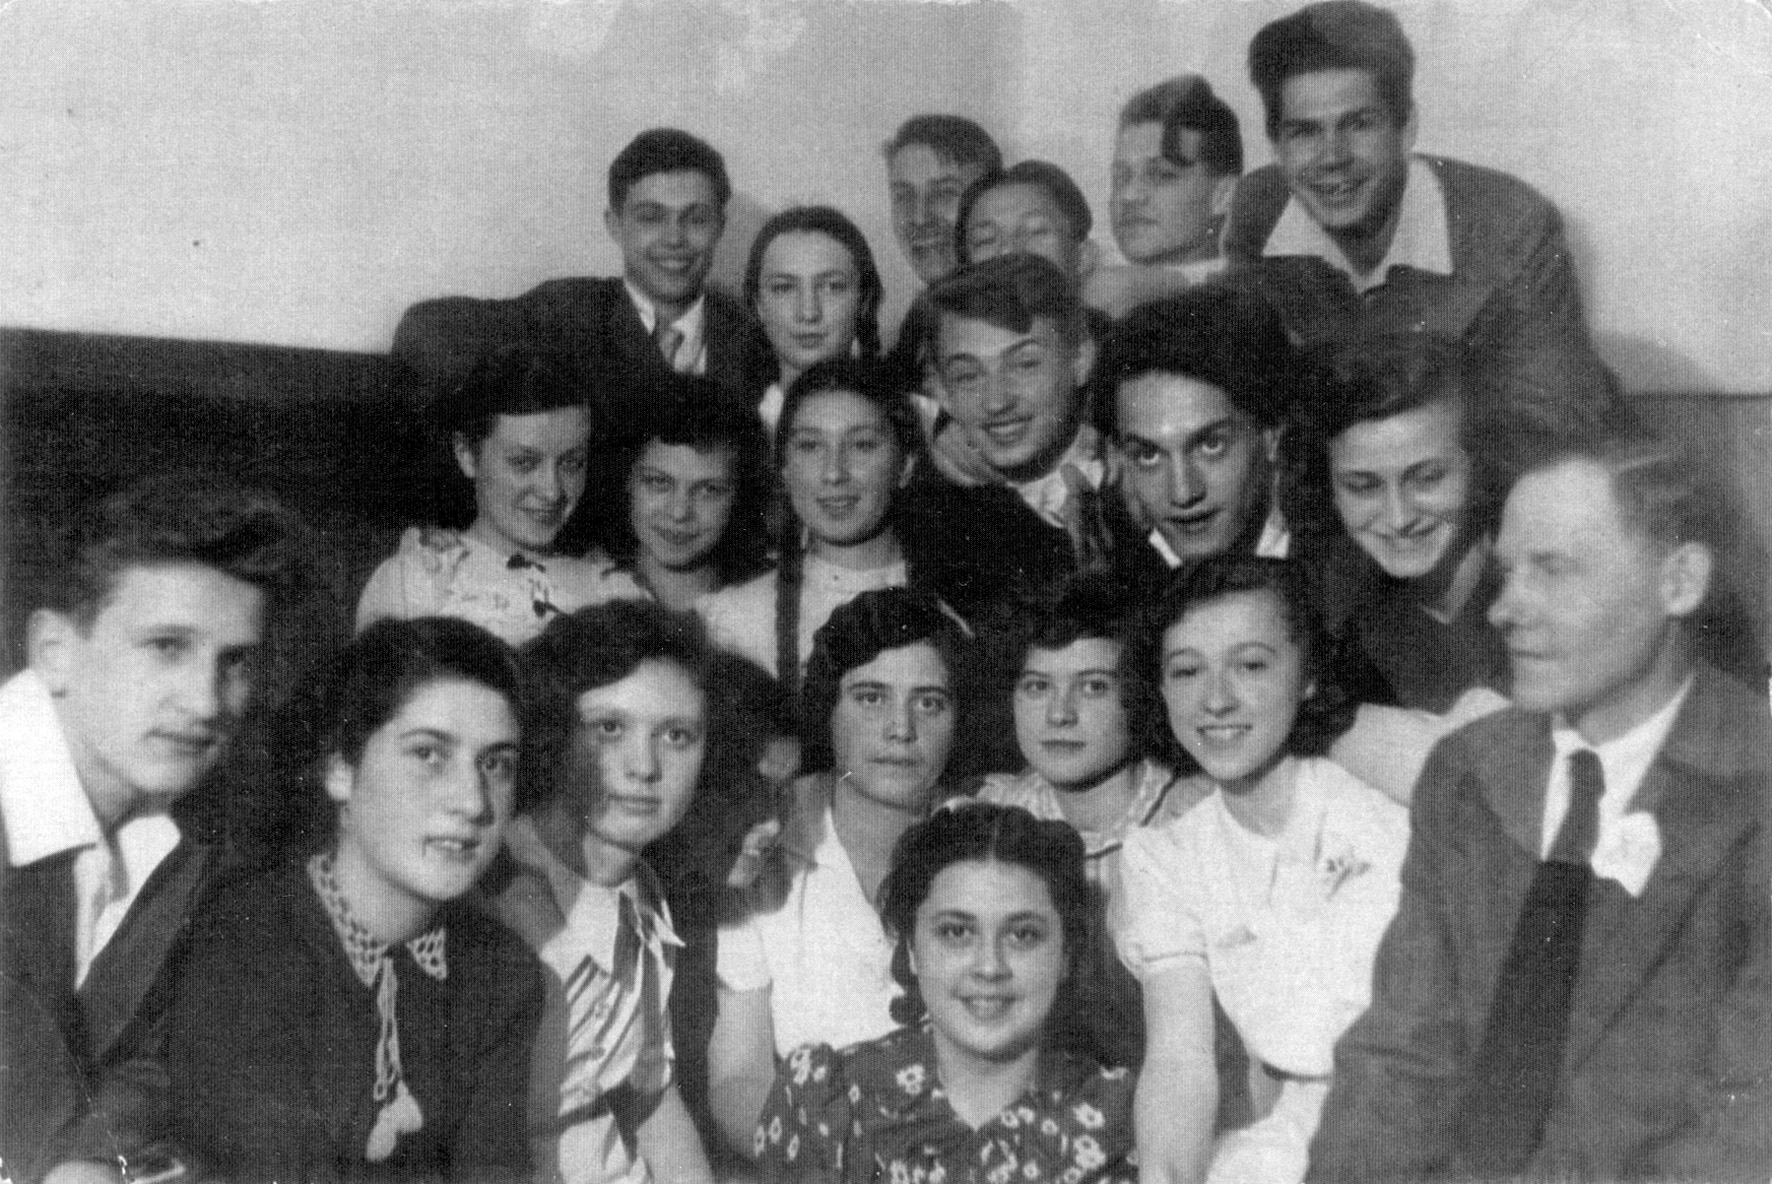
\includegraphics[width=0.5\textwidth]{inc/MalDev}
\end{center}
\begin{center}
    \footnotesize{\textbf {Мальчикам и девочкам 1940-х} \\(1924 года рождения)}
\end{center}

\begin{scriptsize}
\begin{multicols}{2}
    
    \noindent
    К ребятам нашего двора \\
    Пришла не лучшая пора. \\
    \vfill
    \noindent
    Груз годов ведь с плеч не скинешь,\\
    И, куда не поглядишь,\\
    Всюду виден, вроде, фииниш,\\
    И осталось, вроде, шиш! \\
    \vfill
    \noindent
    Только нам, знать, срок не вышел,\\
    Только порох, видно, есть,\\
    Коли вновь мы, братцы, здесь,\\
    Коль мы снова тут, под крышей\\
    Дома номер два дробь шесть.\\
    \vfill
    \noindent
    Откуда шли, шпана дворовая,\\
    Когда пришла пора суровая\\
    Расстаться, шумною толпой\\
    В жизнь, как на праздник~--пей да пой!,--\\
    Ушли веселую шурьбой.\\
    Да каждый со своей судьбой.\\
    \vfill
    \noindent
    Пошли, в цепочку растянувшись,\\
    Один, едва начав, споткнувшись,\\
    Далече не успел уйти\\
    По незавдному пути;\\
    Другой, гляди, взлетел высоко,\\
    А третий ускакал далеко...\\
    \vfill   
    \noindent 
    А мир для всех куда как шире;\\
    В иных домах на нашец жизни ткань:\\
    То~-- шелк с парчей, то~-- просто дрянь!\\
    То планов дрезких грамадье,\\
    То только старое тряпье.\\
    \vfill
    \noindent
    Но жизнь~-- от Бога и надолго.\\
    И не забыть бы, братцы, долга\\
    За нами~-- тем, кто нас родил,\\
    Да тем, кто раньше уходил.\\
    Но не в прекрасную страну,\\
    А на проклятую войну.\\
    \vfill
    \noindent
    Утащила злая баба,\\
    Уложила в поле сдуру\\
    Твоео братишку Абу,\\
    Моего братана Юру,\\
    Сколько было их~-- не счесть!\\
    Всех помянем благородно,\\
    Отдадим посмертно честь!\\
    \vfill
    \noindent
    С непкурытой головою,\\
    То ли лысой, то ль седою,\\
    Постоим да помолчим.\\
    А потом уж прокричим\\
    Из последних сил, что есть,\\
    Славу дому два дробь шесть!\\
\end{multicols}
\end{scriptsize}
\vspace*{-5mm}

{\raggedleft С. И. Д. (Дивильковский С. И.), 2010 г. }


\begin{figure}[ht]
    \begin{minipage}[h!]{40mm}
        \center{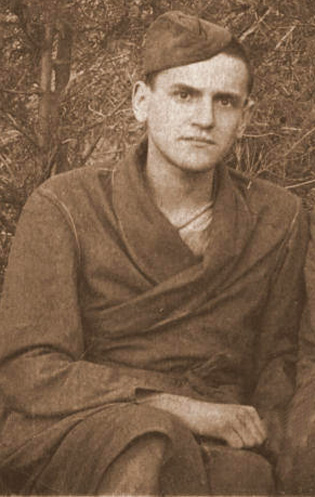
\includegraphics[width=\linewidth]{inc/24} }
    \end{minipage}
    \hfill
    \begin{minipage}[h!]{40mm}
        \center{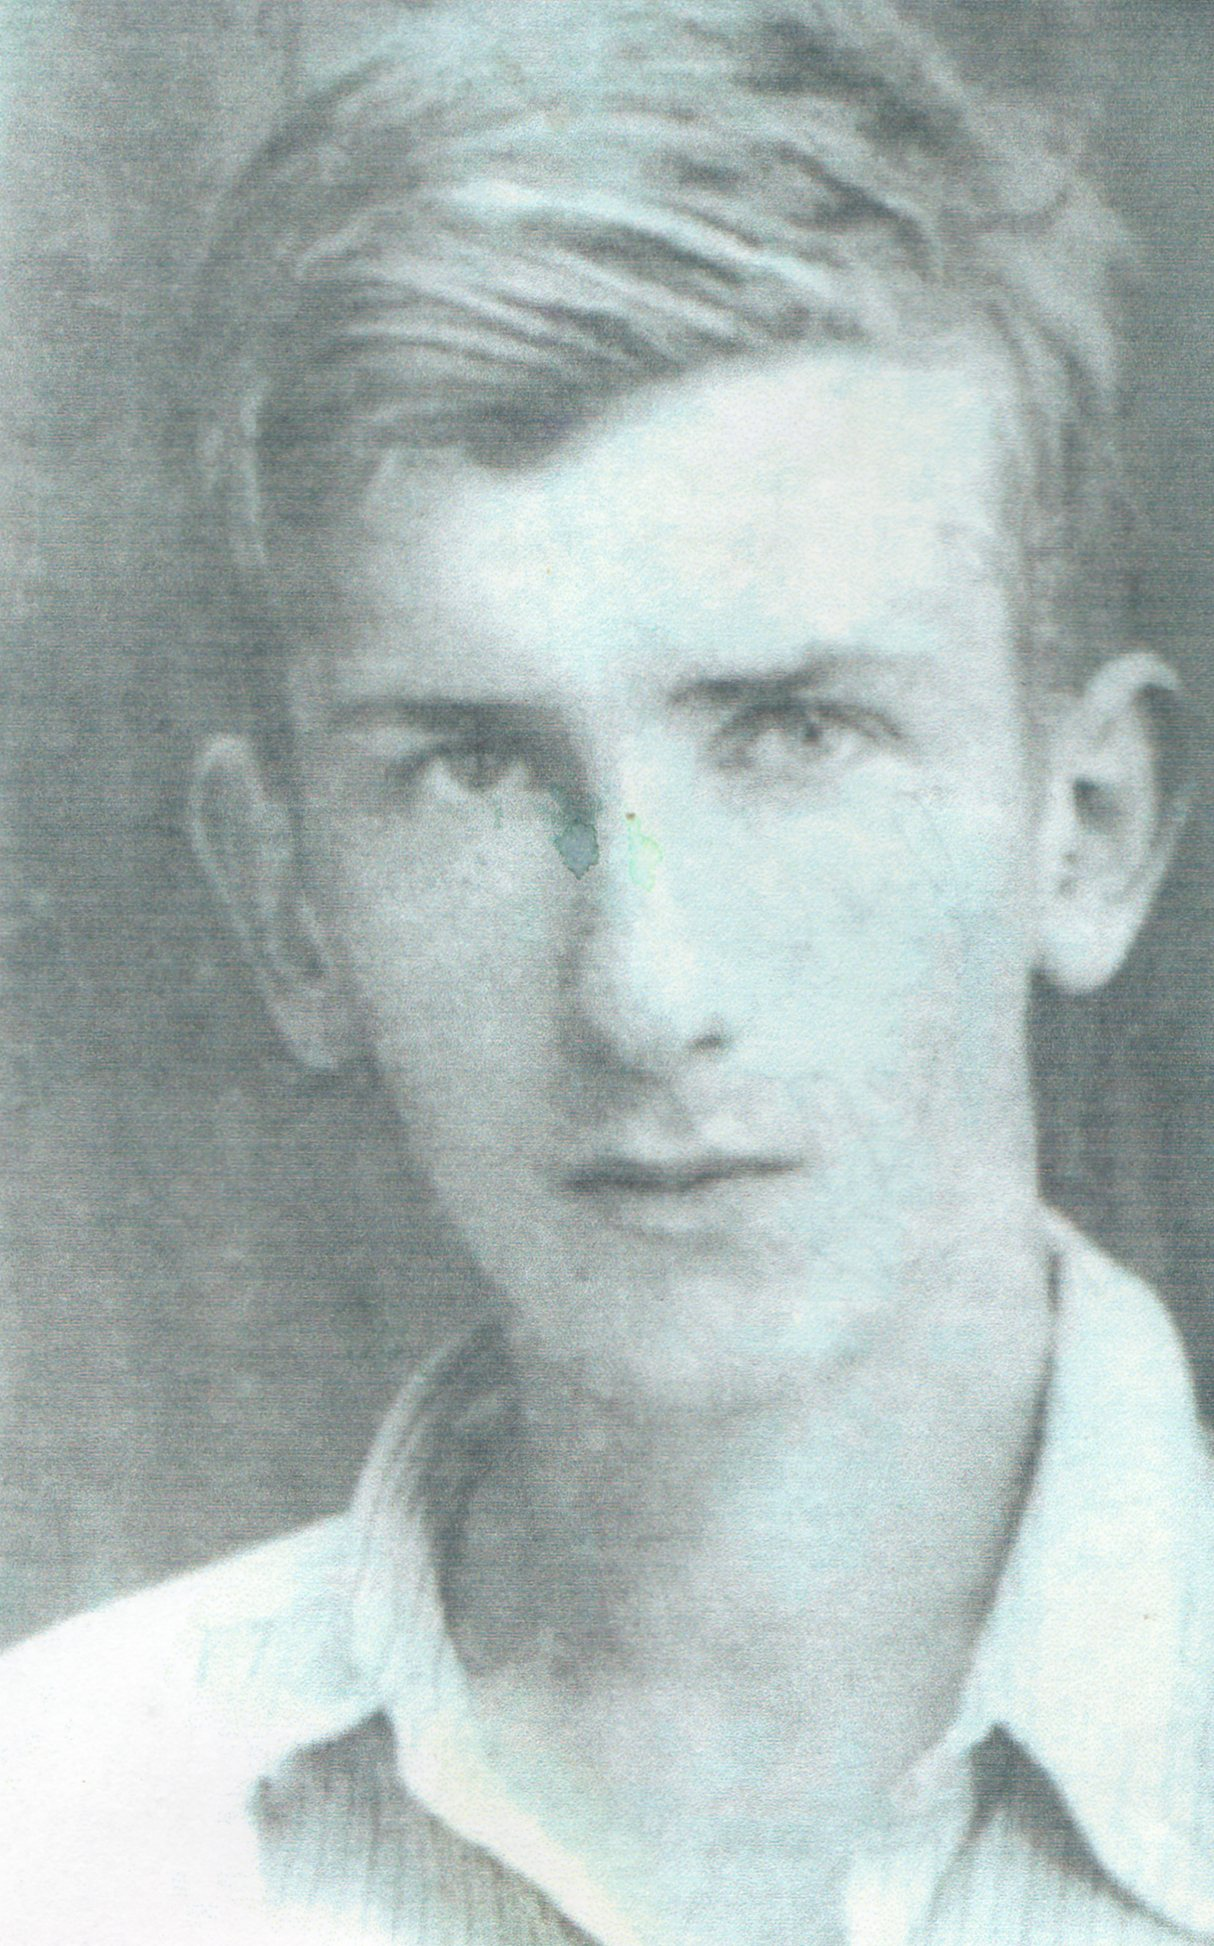
\includegraphics[width=\linewidth]{inc/RG027} }
    \end{minipage}    
    \vspace{-20pt}
    \caption{Аба Миникс и Юра Дивильковский погибли на войне}
\end{figure}

\begin{figure}[h!]
    \begin{minipage}[h!]{40mm}
        \center{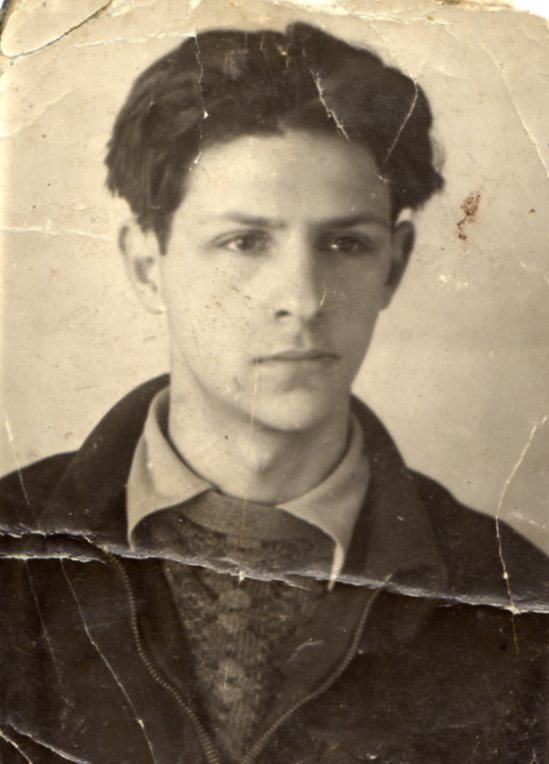
\includegraphics[width=\linewidth]{inc/RG024} }
    \end{minipage}
    \hfill
    \begin{minipage}[h!]{40mm}
        \center{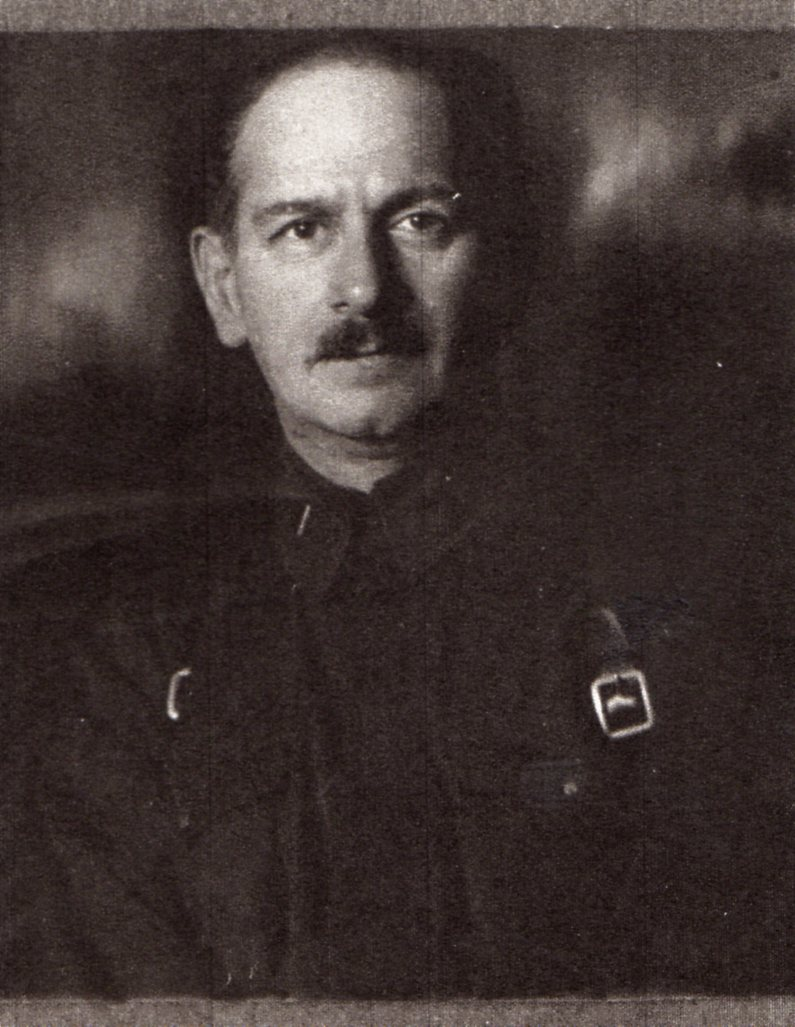
\includegraphics[width=\linewidth]{inc/RG026} }
    \end{minipage}
    \vspace{-20pt}
    \caption{Отец и сын Короткины. Воевали на разных фронтах. Переписывались. Жора погиб. Отец выжил.}
\end{figure}


\begin{figure}
\fcapside{\caption{Сева Варзар прошел всю войну, Жора Короткин~-- погиб.}}{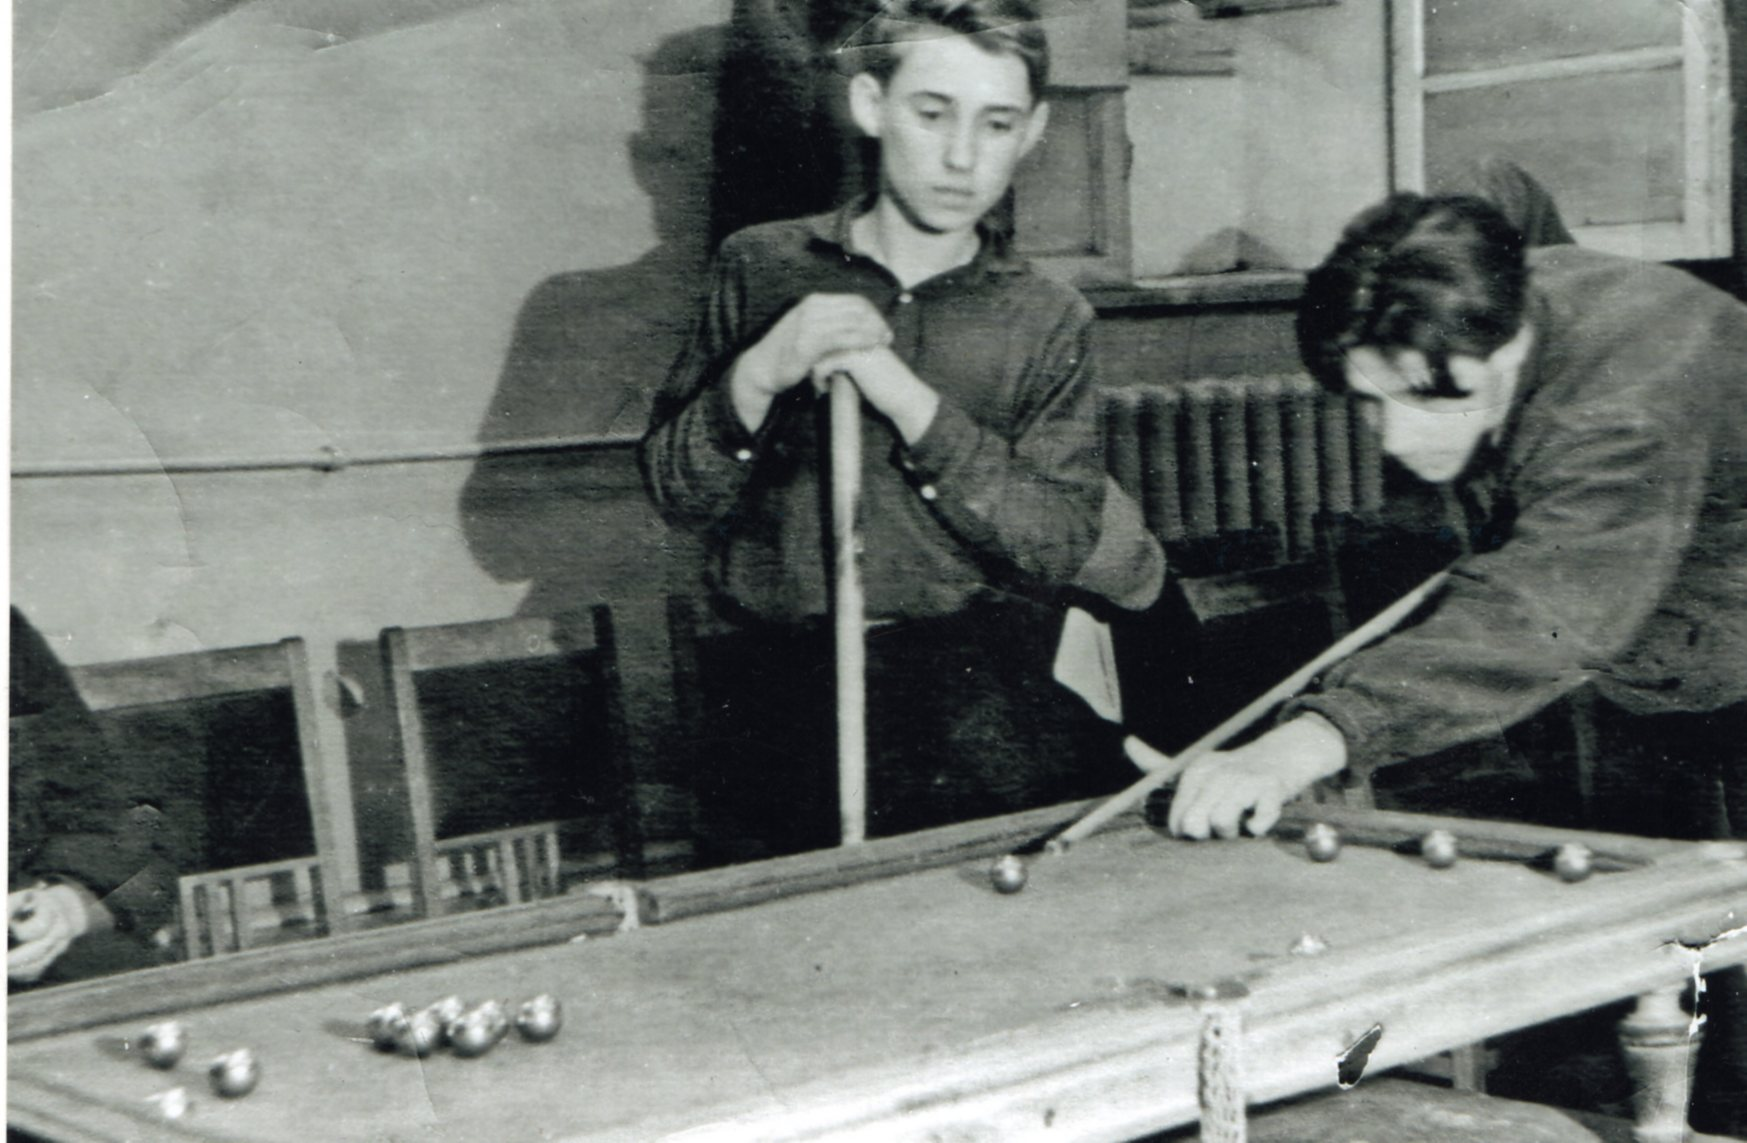
\includegraphics[width=0.5\textwidth]{inc/RG025}}
\end{figure}

\restoregeometry

Особенно ярко эта тенденция проявилась в послевоенные годы. Например, у ребят 1930 года рождения Бирюкова Л. (впоследствии зкончила МАИ, работала конструктором), Варзар К. (инженер-геолог ГлавППУ Москвы), Гриневский О. (МГИМО, дипломат), медников М. (), меньшикова Т. В. (МИИТ, экономист МПС)~-- 1-й подъезд; Андреев В. В. (<<Щепка>>, народный артист СССР), Карпужина З. (МИФИ, ядерщик), Петров И. (МИЭИОО, экономист)~-- 2-й подъезд; Гюнтер М. (), Дивильковский С. (МГИМО, работник ЦККПСС), Кузнецов Л. (МХТИ, зав. лаб. ГИАП)~-- 3-й подъезд; Каменская И. (МГУ, журналист, переводчик)~-- 4-й подъезд; Куроптев Р. (МГИМО, журналист)~-- пятый подъезд; Пивень А. (Плехановка, товаровед)~-- 6-й подъезд; Прейс В. и Штернберг А. (медвузы, врачи)~-- 7-й подъезд. Их друзьями из соседних дворов были Голубев В. (военный), Епишкин В. (Торфяной ин-т, инженер-механик), Зайцева Т. (Плехановка, Госплан РСФСР), Литвинов В. (Акад. им. Куйбышева, полковник, строитель), Стояновский М. (), Улитин Ю. (), Фролоа Л. (Архитектурный институт), Фролов Н. ().

Это уникальное содружество близких по духу людей, которые более или менее часто, но с удовольствием продолжают собираться большими группами уже более 65 (шестидесятипяти) лет! Причем на фотографии 2006 года они еще более жизнерадостны, еще больше нравятся друг другу, чем на фото 1946 года. А ведь еще есть фотография 1936 или 1937 года, где в детском саду встретились представители двух будущих компаний Дома у Красных ворот: <<Союза соединенных дворов>> (ССД) и <<Сумасшедшего дома>> (СД).

\newpage

\newgeometry{top=5mm,bottom=0mm}

\thispagestyle{empty} 
\begin{figure}
    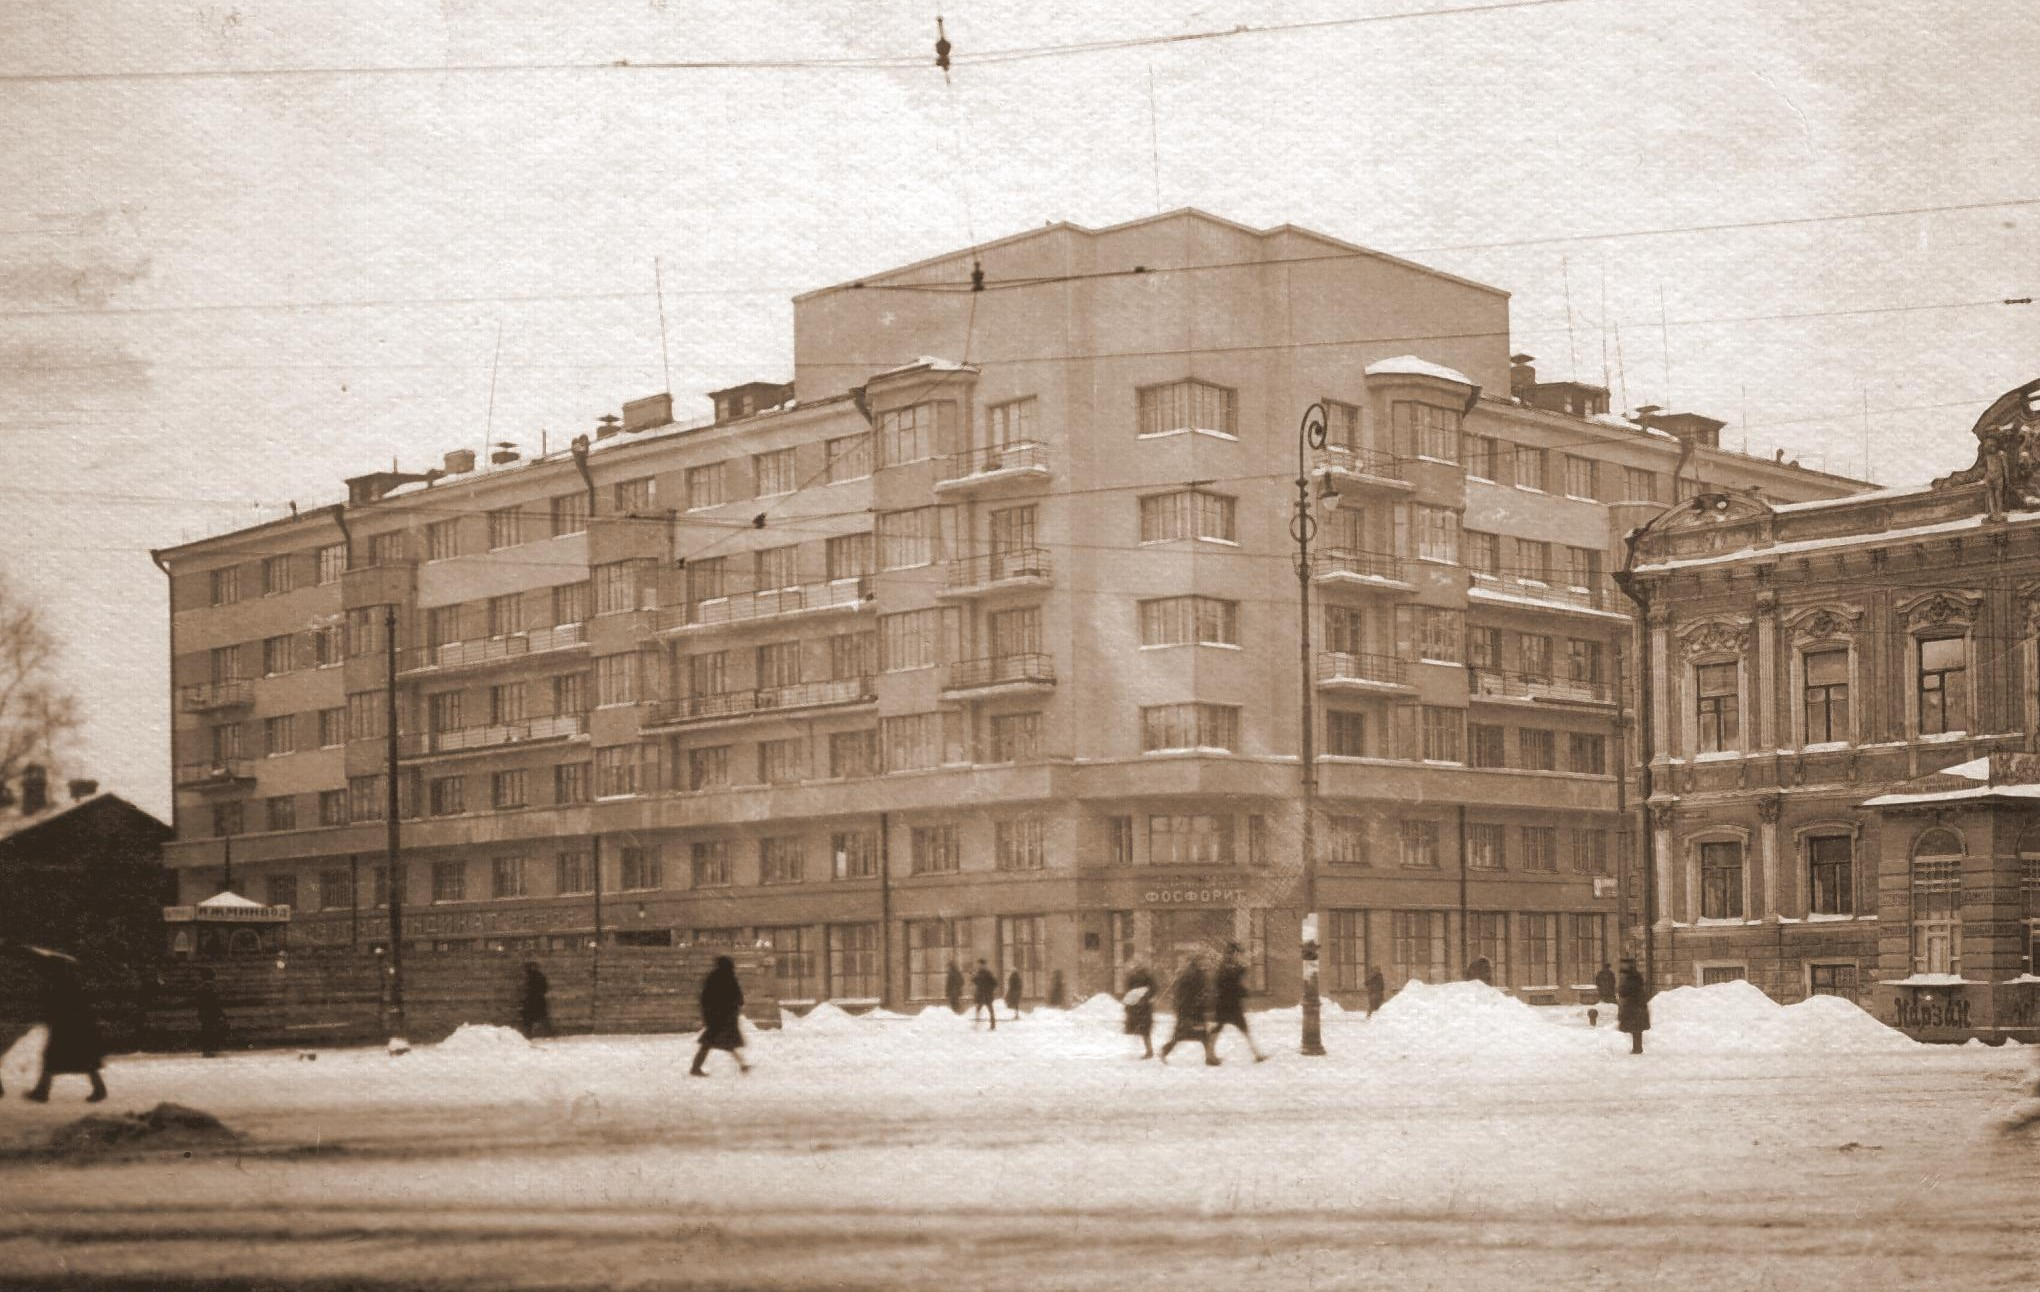
\includegraphics[width=85mm]{inc/2/1}
\end{figure}

\vspace{-20pt}
\vfill

\begin{figure}
    \includegraphics[width=45mm]{inc/2/2}
\end{figure}

\vspace{-20pt}
\vfill
\begin{figure}[h!]
    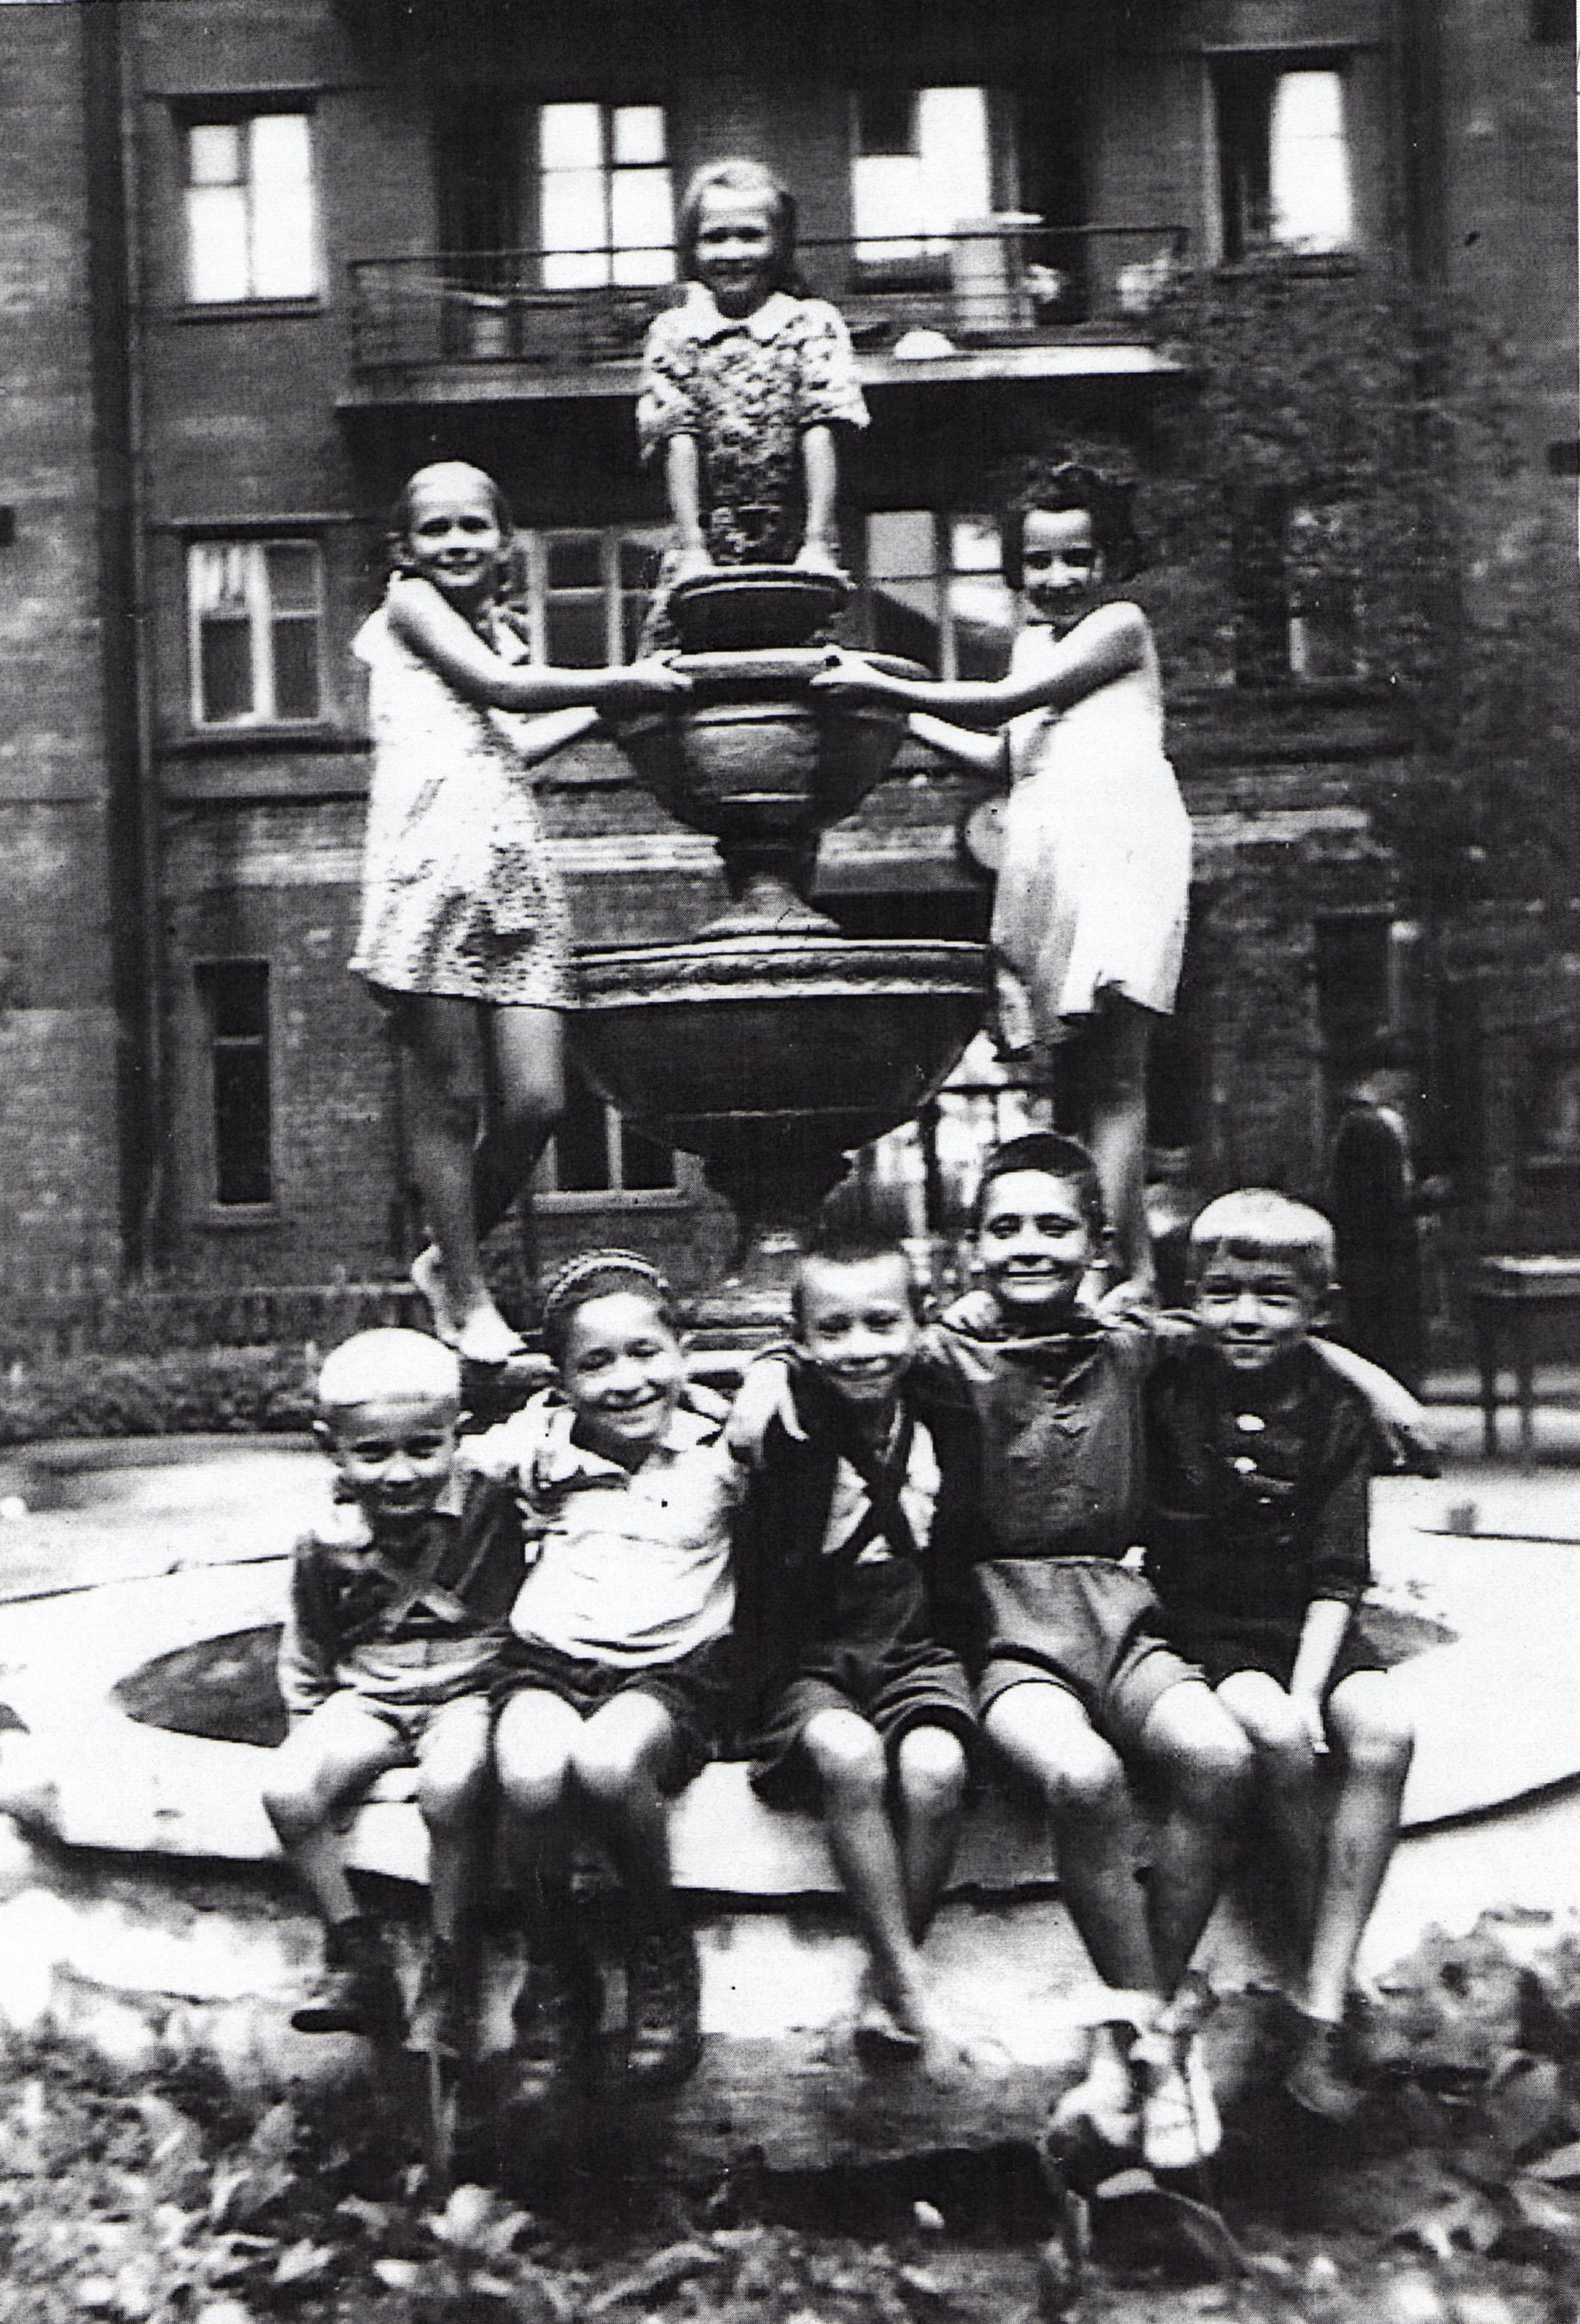
\includegraphics[width=85mm]{inc/2/3}
\end{figure}

\restoregeometry

\begin{figure}
    \caption{Конец 20-х или начало 30-х годов прошлого века. Уже нет людей, которые могли бы сказать, кто есть кто.}
    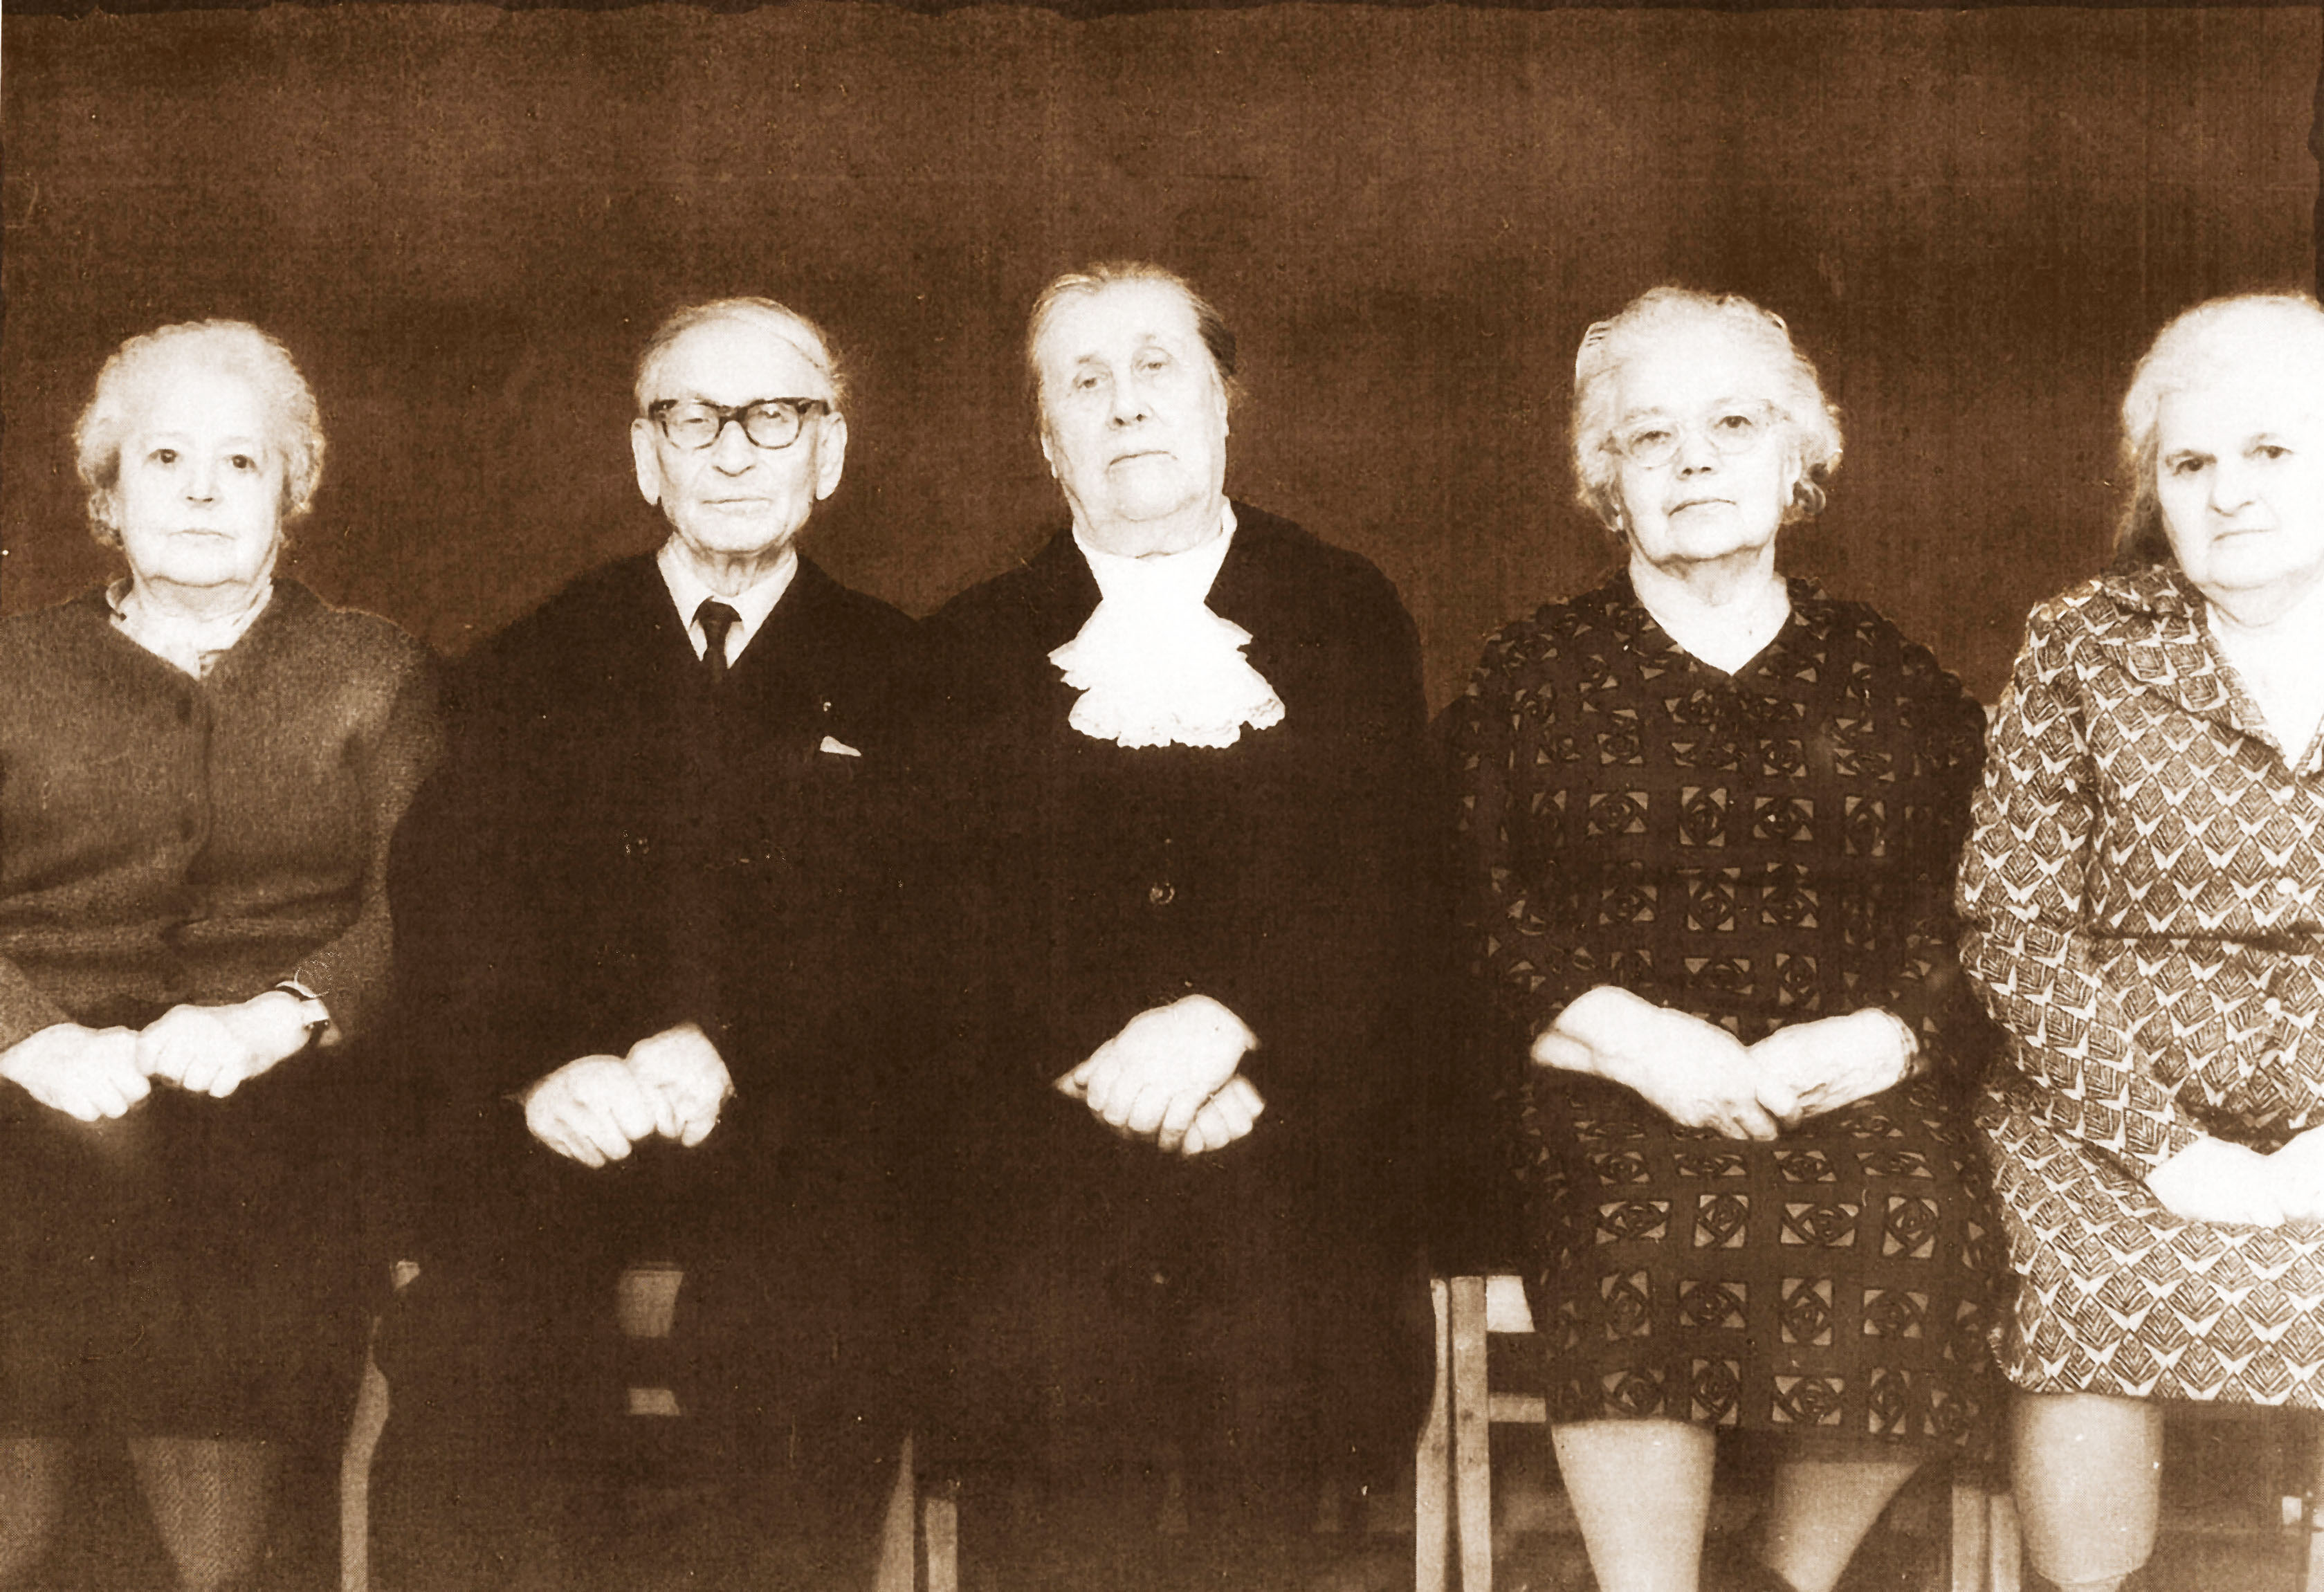
\includegraphics[width=85mm]{inc/3/1}
\end{figure}

\begin{figure}[h!]
    \includegraphics[width=60mm]{inc/3/2}
\end{figure}

\begin{figure}
    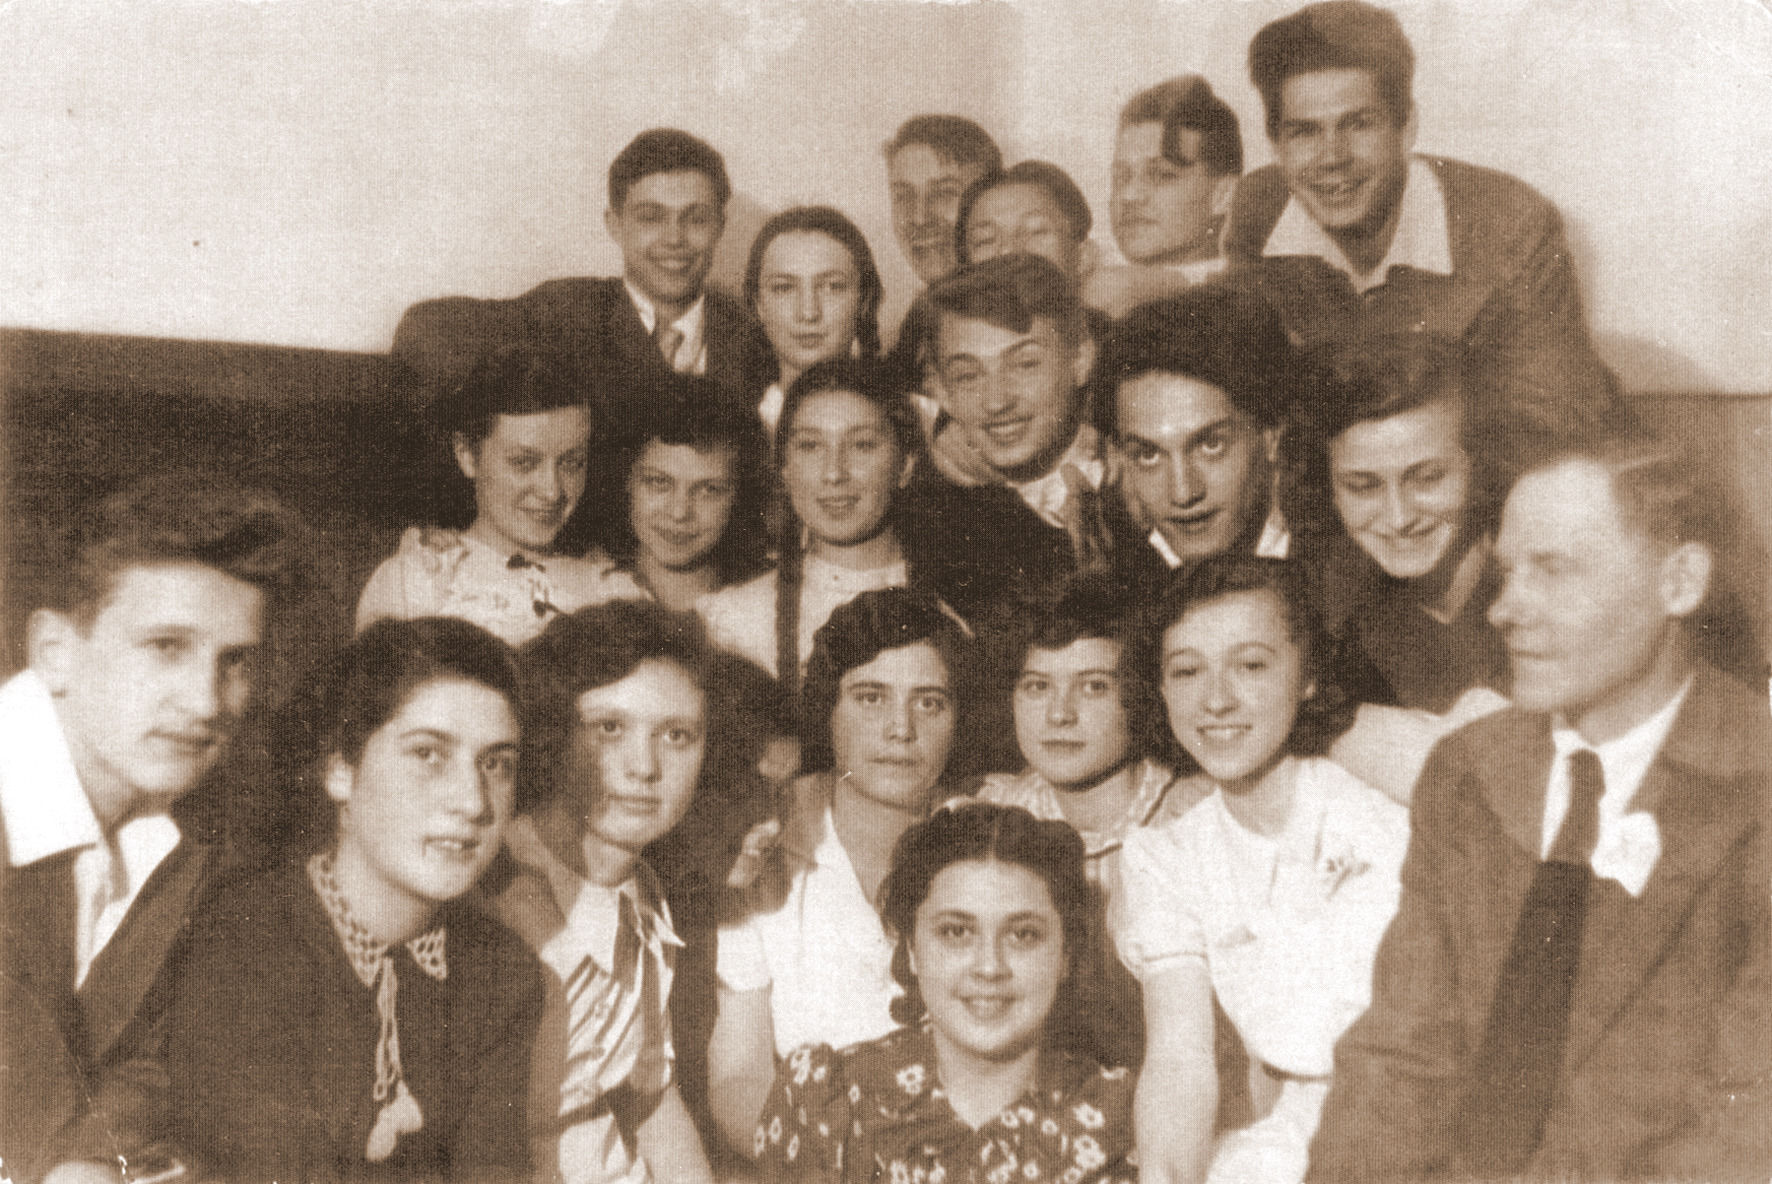
\includegraphics[width=\textwidth]{inc/4/1}
    \caption{ССД 1946г.}
\end{figure}

\begin{figure}[h!]
    \includegraphics[width=\textwidth]{inc/4/2}
    \caption{Борис Коваль, Олегт Гриневский, тамара Зайцева, Наталия N, Леон Кузнецов, Зоя Литвинова (Карпукина), Татьяна Меньшикова накануне всеобщего 80-летия}
\end{figure}
